\chapter{Estudio de Distribución de Carga}
La tercera hipótesis de investigación plantea como responsable del mal rendimiento presentado en el caso de estudio al sistema de gestión y administración de tareas en el sistema operativo. En escenarios multicore como el estudiado, es normal que el sistema operativo realice como procedimiento de rutina la migración de procesos y la re-locación de recursos y datos para evitar la saturación de las componentes del mismo. Un caso práctico de ello es cuando un núcleo de procesamiento está sobre exigido y el sistema operativo redistribuye los procesos que están ejecutándose en dicho núcleo entre los otros procesadores disponibles del sistema con el costo que ello significa. Esta práctica es conocida como \textbf{distribución de carga}, y a pesar de que existen varios mecanismos de aprovechamiento de dicho esquema como una estrategia de balanceo de carga en arquitecturas como la estudiada \cite{paper:NUMA, techsession:numaMemoryThreadsPerformance}, en ciertos escenarios puede degradar el desempeño general del sistema.

Esta hipótesis plantea que dicho proceso de reasignación de recursos sería perjudicial en escenarios de concurrencia sobre arquitecturas como la estudiada, basándose en que mientras un proceso está en plena ejecución, al incorporar más y más tareas en el mismo núcleo de procesamiento agregando nuevos hilos de ejecución, sería el sistema operativo quien comenzaría la reasignación automática de dichos hilos entre los distintos procesadores cayendo en problemas como perdida de referencias de memoria en niveles de caché primario, yendo así en contra del principio de localidad de acceso a la memoria. En su peor escenario, esta teoría lleva al ya mencionado problema de \emph{caché bouncing} que corresponde al fenómeno de sobre corrección de los datos a nivel de líneas de cache de un procesador, producido por constantes cambios de contexto del \emph{scheduller} que genera migración de procesos. Un problema que ya se mencionó en el estudio de la sección previa.

Una alternativa que se ha estudiado para solventar este problema es la técnica de \emph{Processor Affinity} que consiste en la asociación de tareas o procesos en CPUs específicas, de manera de controlar la ubicación de memoria y zona real de ejecución del código en la máquina.
\begin{defn}[ver \cite{article:processoraffinity}] \textbf{Processor Affinity} es una estrategia de trabajo que consiste en la asociación de ciertos procesos o hilos de trabajo con determinados núcleos de procesamiento lógicos de un sistema. Dicha asociación restringe la capacidad de ejecución del hilo o proceso exclusivamente a su núcleo de procesamiento asignado.
\end{defn}
En otras palabras, con la aplicación de \emph{processor affinity} se remueve la utilidad del mismo scheduler del sistema operativo para coordinar la mejor operación en la asignación de los hilos de ejecución a las distintas CPU disponible, reemplazándolo por un criterio de diseño humano construido consientes de la tarea que se desea realizar. Es una técnica muy ambiciosa en el sentido de que bien empleada puede proveer muy buenos resultados en el sistema \cite{paper:cacheaffinity}, sin embargo, es muy fácil errar al interpretar el diseño de operación que se desea coordinar, llevando a una mala implementación en la asignación de recursos que termina degradando fuertemente el desempeño del sistema completo.

En este tercer estudio se plantea la utilización de la técnica de \emph{processor affinity} en pos de conseguir un mejor rendimiento del caso de estudio presentado, ello por medio de la reasignación de los hilos de ejecución entre los distintos cores lógicos del sistema en pos de explotar mejor la localidad de recursos en una arquitectura como la que se dispone. Para evaluar lo anterior, se plantean distintos esquemas de asignación de recursos basados en argumentos arquitecturales del escenario de prueba y se evalúan comparativamente los resultados.

\section{Esquemas de Distribución}
Se diseñaron variados esquemas de asignación a fin de evaluar distintos enfoques de aprovechamiento del principio de localidad de memoria. En total se diseñaron 6 esquemas para evaluar combinaciones dinámicas de cores lógicos reconocidos por el sistema operativo en búsqueda de mejores rendimientos. Los esquemas se detallan a continuación:
\begin{description}
\item[Sin Processor Affinity] Asignación dinámica por el scheduller del sistema operativo. En este caso, la elección la hace el sistema de acuerdo a complejos algoritmos que consideran prioridad de proceso, carga de CPU, entre otros. Sirve como punto base de comparación con respecto a los demás esquemas.
\item[DummyAffinity] Asignación directa de hilos a ejecución en el core 0 del sistema, así, todos los hilos se delegan al mismo core. Bajo este esquema se presume que se puede aprovechar mejor la localidad de memoria al disponer en el banco de memoria más próximo al núcleo de ejecución todas las referencias necesarias, disminuyendo el efecto de sobrecarga de los protocolos de coherencia y coordinación de cache.
\item[EquitativeAffinity] Asignación secuencial equitativa entre los cores lógicos del sistema siguiendo la numeración que el sistema operativo dispone de los núcleos mismos. Supone que la distribución completamente justa y equitativa entre cores entrega un mejor rendimiento general al reducir la carga de procesamiento de cada core.
\item[PairAffinity] Asignación secuencial de hilos a cores de numeración par. Busca descartar un escenario donde los cores duplicados por efecto de la tecnología \emph{hyperthreading} de Intel pudieran no aprovechar cores reales, generando así un mejor desempeño final.
\item[ImpairAffinity] Asignación secuencial de hilos a cores de numeración impar. Similar al anterior variando los cores elegidos.
\item[NumaPairAffinity] Asignación de los hilos a cores del segundo conjunto NUMA disponible en el sistema. Sigue la idea de aprovechar toda una unidad lógica de procesamiento según la arquitectura \emph{Quickpath}, persiguiendo mejores tiempos al tener mejor acceso a memoria desde éstos cores.
\item[SimpleCoreAffinity] Asignación de los hilos a los primeros dos cores lógicos del sistema, correspondientes al primer core real duplicado por efecto \emph{HyperThreading}.
\end{description}

\begin{table}[]
\centering
\begin{tabular}{|l|l|}
\hline
\multicolumn{1}{|c|}{\textbf{Esquema}} & \multicolumn{1}{c|}{\textbf{Fórmula de numeración de afinidad por hilos}}                                  \\ \hline
DummyAffinity                          & 

$\displaystyle 0$
                                                                                            \\ \hline
EquitativeAffinity                     & $\displaystyle i+1 \pmod \Phi $                                                                                 \\ \hline
PairAffinity                           & $\displaystyle 2i \pmod \Phi $                                                                                 \\ \hline
ImpairAffinity                         & $\displaystyle 2i + 1 \pmod \Phi $                                                                               \\ \hline
SimpleCoreAffinity                     & $\displaystyle \frac{i \pmod 2}{2} \Phi$                                                                              
\\ \hline
NumaPairAffinity                       & 
$
\begin{cases}
    \displaystyle i \pmod \Phi & \displaystyle \text{si } i \pmod 2 = 0 \\
    \displaystyle (i-1) + \frac{\Phi}{2} \pmod \Phi & \displaystyle \text{si } i \pmod 2 \neq 0
\end{cases}
$ \\ \hline
\end{tabular}
\caption{Numeración de afinidad a cada hilo en ejecución, donde $i$ representa el i-ésimo hilo. y $\Phi$ corresponde al número de procesadores lógicos reconocidos en el sistema (24 para nuestro caso).}
\label{my-label}
\end{table}

Con los esquemas antes mostrados, se pretende explotar las bondades de la arquitectura NUMA, de los principios de localidad de memoria, y de proximidad de acceso en los datos, a través de una ganancia efectiva en los tiempos de la prueba del caso de estudio.

\section{Metodología de Experimentación}
Para evaluar los distintos esquemas de afinidad ya postulados, se modificó el caso de estudio para incorporar la asociación de hilos de ejecución para con los distintos cores del sistema. Para ello se aprovechó la flexibilidad de la librería \emph{PThreads}, responsable de brindar los hilos de ejecución en nuestro caso, para usar ciertas llamadas a sistema que nos otorgasen el control de la localidad de ejecución buscada. En concreto, se empleó la función \verb=pthread_attr_setaffinity_np()= que permite especificar precisamente la asociación de un hilo para con el core de ejecución deseado. 

La prueba anterior se recopiló en un nuevo experimento\footnote{\url{https://github.com/sebablasko/Test_DifferentAffinityThreadsBySocket}} que, para efectos de validez estadística, se ejecutó un total de 60 veces, y se rescataron los valores promedios de dichas ejecuciones, ello siguiendo las mismas lógicas de colección de datos del promedio de las ecuaciones \ref{eq:tupla1} y \ref{eq:promedio}.

\newpage

\section{Resultados}

\begin{figure}[h!]
	\centering
	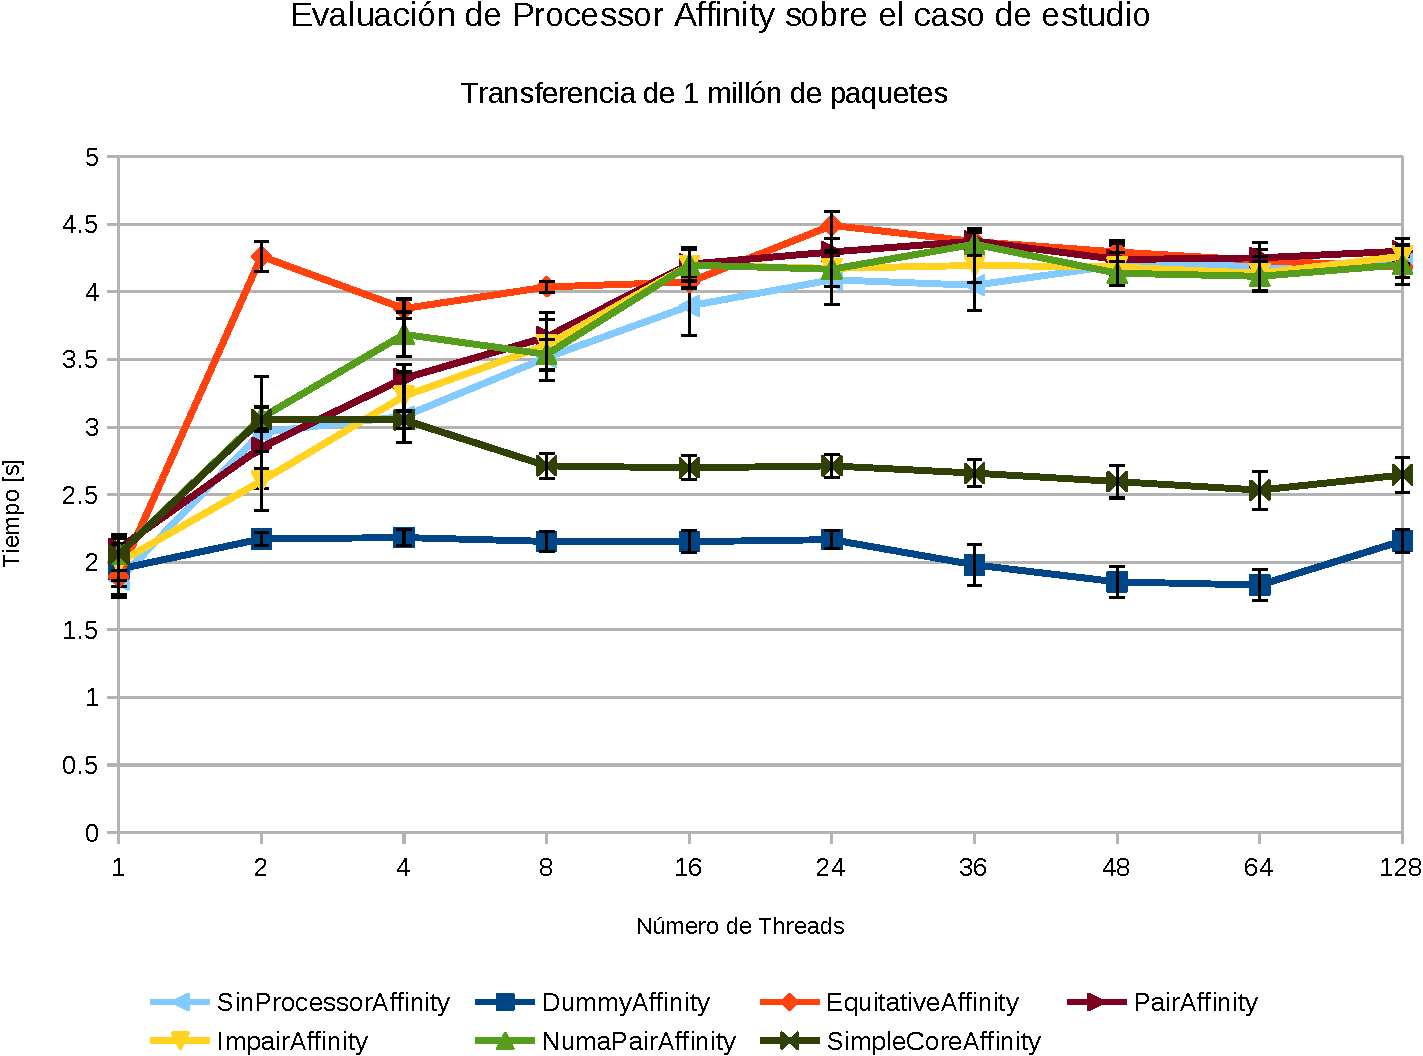
\includegraphics[scale=.6]{resultados/processoraffinity-crop.pdf}
	\caption{Resultados experimentales de los distintos esquemas de afinidad.}
	\label{fig:resAffinity}
\end{figure}

\section{Análisis y Discusión de Resultados}
Los resultados experimentales ilustrados en la figura \ref{fig:resAffinity} son diversos. En efecto, ningún esquema de distribución evaluado consiguió reducir verdaderamente el tiempo de ejecución con respecto al uso de una configuración trivial de un único thread. Sin embargo los resultados obtenidos reflejan distintas tendencias interesantes en los tiempos resultantes del experimento.

Una primera tendencia evidenciada en los resultados viene dado por los esquemas \textbf{DummyAffinity} y \textbf{SimpleCoreAffinity}, donde los tiempos se mantuvieron estables a lo largo de la evaluación de las distintas configuraciones de threads. Si recordamos, ambos esquemas son rígidos en la posibilidad de locación de los hilos en la CPU, el primero los asigna todos al core \#0 mientras que el segundo los asigna todos entre el core \#0 y el core \#12, numeración que da el sistema operativo a los núcleos duplicados por efecto de la tecnología \emph{HyperThreading}. De ésta manera, ambos esquemas tienen en común que ejecutan la totalidad de los hilos en un mismo núcleo real de procesamiento. Ahora bien, ninguno de los dos consigue ganancias efectivas de tiempo con respecto al uso de un único thread, ello se explica pues, dado que los distintos hilos son asignados todos a un mismo core, la ejecución de los mismos termina degenerando a una ejecución secuencial, es decir, por medio de la afinidad de proceso hemos eliminado la capacidad de paralelismo al llevar el experimento a un escenario monocore. Esto explica también el por qué los tiempos son tan uniformes sin importar la cantidad de hilos que se usen.

Una segunda tendencia reconocible es la ilustrada por el esquema \textbf{EquitativeAffinity}. Resultante como el de peor desempeño, este esquema que se caracterizaba por la distribución justa de los hilos entre los cores registra siempre los peores tiempos de la prueba. Esta tendencia se explica por la naturaleza de la arquitectura que se está usando. Como se mencionó antes, la distribución del sistema corresponde a dos nodos NUMA de procesamiento. La aplicación del esquema equitativo vulnera derechamente tanto los beneficios que provee el esquema NUMA como el principio mismo de localidad en acceso a la memoria, ello pues en la práctica, termina distribuyendo los distintos hilos en las componentes más alejadas (topológicamente) de la arquitectura disponible.

Finalmente, una tercera tendencia es la de crecimiento producido por el conjunto de los demás esquemas de afinidad. La similitud entre \textbf{PairAffinity} e \textbf{ImpairAffinity} era previsible pues el modelo de distribución era equivalente para ambos. La misma naturaleza sigue el esquema \textbf{NumaPairAffinity} que, a pesar de aprovechar la distribución de componentes para la localización de hilos, no consiguió mejores tiempos que los ya representados. Ahora bien, hay que destacar que en términos prácticos, este último grupo de esquemas de distribución tuvo un rendimiento muy similar al del mismísimo scheduller del sistema operativo, más aún, con la técnica de \emph{processor affinity}, la ejecución del programa es rígida en la localidad del proceso con respecto al procesador seleccionado, lo cual produce que en ciertas situaciones --como al tener sobrecarga de memoria-- los niveles de caché no cooperen con la tarea general, y no brinden mayor beneficio a la prueba final, una garantía que sí dispone el scheduller del sistema operativo, por lo tanto su desempeño no debe ser menospreciado y sólo da cuenta de que lamentablemente, el problema de rendimiento parece ser producto de un defecto de diseño inherente a la estructura que se está compartiendo, defecto que no permite optar a mejores tiempos sin importar la estrategia de paralelismo usada.


\section{Conclusiones}
A raíz del estudio de distribución de carga se pueden rescatar varios aspectos interesantes:
\begin{itemize}
\item Las técnicas de \emph{processor affinity} empleadas no consiguieron beneficio alguno en el rendimiento de consumo del caso de estudio, ello a pesar de evaluar distintos esquemas en pos de sacar provecho de la arquitectura evaluada.
\item Los distintos esquemas, a pesar de ser rígidos en la ejecución de hilos sobre ciertos cores, fueron competitivos con respecto a la capacidad dinámica del scheduller del sistema operativo en los tiempos producidos en el experimento.
\item Se determina que es el mismo socket –o alguna componente inherente de sincronización como su spinlock-- una estructura que se vuelve un punto de contención al emplear hilos paralelos, calificando al mismo como no apto para soportar accesos concurrentes, ello dado su diseño y mecanismos de protección implementados.
\end{itemize}